%\newcommand{\sms}{\mathbf{S}}

\chapter{Material File Command Reference}\label{chap:MaterialFileCommandReference}
The material file defines all the magnetic properties of the materials used in
the simulation, including exchange, anisotropy, damping etc. Material properties
are defined by an \textit{index} number for each material, starting at one.
Material properties are then defined as follows:

\textit{material[index]:keyword = value !unit}

\noindent followed by a carriage return, so that each property is defined on a
separate line. The defined keywords are listed below. The material file is
largely free-format, apart from the first line which must specify the number of
materials for the simulation. The material properties can be defined in any
order, and if omitted the default value will be used. When the same property
for a particular material is defined in the file, the last definition (reading
top to bottom) will be used. Comments can be added to the file using the \#
character, which moves the file parser to the next line.

\section*{Material File Parameters}
\phantomsection\addcontentsline{toc}{section}{Material File Parameters}

{\zicf material:num-materials = int [1-100; default 1]}
\phantomsection\addcontentsline{toc}{subsection}{material:num-materials}
Defines the number of materials to be used in the simulation, and must be the
first uncommented line in the file. If more than $n$ materials are defined, then
only the first $n$ materials are actually used. The maximum number of different
materials is currently limited to 100. If using a custom unit cell then the
number of materials in the unit cell cell must match the number of materials
here, otherwise the code will produce an error.

{\zicf material:material-name = string [default material\#n]}
\phantomsection\addcontentsline{toc}{subsection}{material:material-name}
Defines an identifying name for the material with a maximum length of xx
characters. The identifying name is only used in the output files and does not
affect the running of the code.

{\zicf material:damping-constant = float [0.0-10.0; default 1.0]}
\phantomsection\addcontentsline{toc}{subsection}{material:damping-constant}
Defines the phenomenological relaxation rate (damping) in dynamic simulations
using the LLG equation. For equilibrium properties the damping should be set
to 1 (critical damping), while for realistic dynamics the damping should be
representative of the material. Typical values range from 0.005 to 0.1 for most
materials.

{\zicf material:exchange-matrix[index] = float [default 0.0 J/link]}
\phantomsection\addcontentsline{toc}{subsection}{material:exchange-matrix}
Defines the pairwise exchange energy between atoms of type index and
neighbour-index. The pair wise exchange energy is independent of the
coordination number, and so the total exchange integral will depend on the
number of nearest neighbours for the crystal lattice. The exchange energy must
be defined between all material pairs in the simulation, with positive values
representing ferromagnetic coupling, and negative values representing
anti-ferromagnetic coupling. For a ferromagnet with nearest neighbour exchange,
the pairwise exchange energy can be found from the Curie temperature by the
mean-field expression:

\begin{equation*}
\Jij = \frac{3\kB\Tc}{\epsilon z}
\end{equation*}

\noindent where $\Jij$ is the exchange energy, $\kB$ is the Boltzmann constant,
$\Tc$ is the Curie temperature, $z$ is the coordination number (number of
nearest neighbours) and $\epsilon$ is a correction factor to account for spin
wave fluctuations in different crystal lattices. If a custom unit cell file
with non-normalised exchange interactions is used the exchange values defined
here are ignored.

{\zicf material:exchange-matrix-1st-nn[index] = float [default 0.0 J/link]}
\phantomsection\addcontentsline{toc}{subsection}{material:exchange-matrix-1st-nn}
Defines the pairwise exchange energy between atoms of type index and
neighbour-index for the first nearest neighbour shell when using the built in
exchange functions. This is exactly the same as the usual parameter
exchange-matrix[index] but with a more specific syntax including the shell
number of 1.

{\zicf material:exchange-matrix-2nd-nn[index] = float [default 0.0 J/link]}
\phantomsection\addcontentsline{toc}{subsection}{material:exchange-matrix-2nd-nn}
Defines the pairwise exchange energy between atoms of type index and
neighbour-index for the second nearest neighbour shell when using the built in
exchange functions. If you are using the generic crystal structures available
in \vampire, then it is possible to define a longer ranged Hamiltonian with
next-nearest up to 10th nearest neighbour interactions. The interaction shells
refer to sets of neighbours with the same interaction range from a target atom.
To define a longer range Hamiltonian you need to define the input file
parameters  textit{exchange:interaction-range = $R$} and
\textit{exchange:function = shell}, where $R$ is the interaction range as a
multiple of the nearest neighbour distance. When these options are defined, the
number of computed shells is printed in the log file along with their distance
and coordination number. For the common crystal structures the shell
coordinations are well know. Note that longer ranged Hamiltonians will naturally
be slower due to the larger number of computed exchange interactions. For more
than ten shells or asymmetric crystals with different interactions along
different crystal directions the unit cell file is still required.

{\zicf material:exchange-matrix-3rd-nn[index] = float [default 0.0 J/link]}
\phantomsection\addcontentsline{toc}{subsection}{material:exchange-matrix-3rd-nn}
Defines the pairwise exchange energy between atoms of type index and
neighbour-index for the third nearest neighbour shell when using the built in
exchange functions. See 2nd neighbour description for more details on using
this feature.

{\zicf material:exchange-matrix-(4th-10th)-nn[index] = float [default 0.0 J/link]}
\phantomsection\addcontentsline{toc}{subsection}{material:exchange-matrix-4th-nn}
Defines the pairwise exchange energy between atoms of type index and
neighbour-index for the fourth nearest neighbour shell when using the built in
exchange functions. See 2nd neighbour description for more details on using this
feature.

{\zicf material:biquadratic-exchange-matrix[index] = float [default 0.0 J/link]}
\phantomsection\addcontentsline{toc}{subsection}{material:biquadratic-exchange-matrix}
Defines the pairwise biquadratic exchange energy between atoms of type index and
neighbour-index. The pair wise exchange energy is independent of the
coordination number, and so the total exchange integral will depend on the
number of neighbours for the crystal lattice. The exchange energy must be
defined between all material pairs in the simulation, with positive values
representing ferromagnetic coupling, and negative values representing
anti-ferromagnetic coupling. The biquadratic exchange Hamiltonian is given by
the expression

\begin{equation*}
E^{\mathrm{BQ}} = \sum_{i<j} \Jij^{\mathrm{BQ}} \left( \sms_i \cdot \sms_j \right)^2
\end{equation*}

\noindent where $\Jij^{\mathrm{BQ}}$ is the biquadratic exchange energy.
%{\zicf material:total-exchange-matrix[j] = float [default 12x5.6 J/link]}

{\zicf material:atomic-spin-moment = float [0.01+ \muB, default 1.72 \muB]}
\phantomsection\addcontentsline{toc}{subsection}{material:atomic-spin-moment}
Defines the local effective spin moment for each atomic site. Atomic moments
can be found from ab-initio calculations or derived from low temperature
measurements of the saturation magnetisation. The atomic spin moments are
related to the macroscopic magnetisation by the expression:

\begin{equation*}
\smmu = \frac{\Ms a^3}{n}
\end{equation*}

\noindent where $a$ is the lattice constant, $n$ is the number of atoms per
unit cell, and \Ms is the saturation magnetisation in units of J/T/m$^3$ (A/m).
Note that unlike micromagnetic simulations, atomistic simulations always use
zero-K values of the spin moments, since thermal fluctuations of the
magnetisation are provided by the model. Small values ($<1 \muB$) will
typically lead to integration problems for the LLG unless sub-femtosecond time
steps are used.

%--------------------------------
% Magnetic anisotropy parameters
%--------------------------------
{\zicf material:uniaxial-anisotropy-constant = float [default 0.0 J/atom]}
\phantomsection\addcontentsline{toc}{subsection}{material:uniaxial-anisotropy-constant}
Defines the local second order single-ion magnetocrystalline anisotropy constant
at each atomic site. The anisotropy energy is given by the expression

\begin{equation*}
E_i = -\kuu (\sms_i \cdot \ei)^2
\end{equation*}

\noindent where $\sms_i$ is the local spin direction and \ei is the easy axis
unit vector. Positive values of \kuu give a preferred easy axis orientation,
and negative values give a preferred easy plane orientation of the spin
perpendicular to the easy axis direction.

{\zicf material:second-order-uniaxial-anisotropy-constant = float [default 0.0\newline J/atom]}
\phantomsection\addcontentsline{toc}{subsection}{material:second-order-uniaxial-anisotropy-constant}
Has the same meaning and is the preferred form for
material:uniaxial-anisotropy-constant.

{\zicf material:fourth-order-uniaxial-anisotropy-constant = float [default 0.0\newline J/atom]}
\phantomsection\addcontentsline{toc}{subsection}{material:fourth-order-uniaxial-anisotropy-constant}
Implements fourth order uniaxial anisotropy as implemented with spherical
harmonics.

{\zicf material:cubic-anisotropy-constant = float [default 0.0 J/atom]}
\phantomsection\addcontentsline{toc}{subsection}{material:cubic-anisotropy-constant}
Defines the local cubic magnetocrystalline anisotropy constant at each atomic
site. The anisotropy energy is given by the expression

\begin{equation*}
E_i = +\frac{\kc}{2} (S_x^4 + S_y^4 + S_z^4)
\end{equation*}

\noindent where $S_{x,y,z}$ are the components of the local spin direction and
\kc is the cubic anisotropy constant. Positive values of \kc give a preferred
easy axis orientation along the [001] directions, medium-hard along the [110]
directions and hard along the [111] directions. Negative values give a preferred
easy direction along the [111] directions, medium ahead along the [110]
directions and hard along the [100] directions.

{\zicf material:fourth-order-cubic-anisotropy-constant = float [default 0.0\newline J/atom]}
\phantomsection\addcontentsline{toc}{subsection}{material:fourth-order-cubic-anisotropy-constant}
Has the same meaning and preferred form for material:cubic-anisotropy-constant.

{\zicf material:uniaxial-anisotropy-direction = float vector [default (0,0,1)]}
\phantomsection\addcontentsline{toc}{subsection}{material:uniaxial-anisotropy-direction}
A unit vector \ei describing the magnetic easy axis direction for uniaxial
anisotropy. The vector is entered in comma delimited form - For example:

\textit{material[1]:uniaxial-anisotropy-direction = 0,0,1}

\noindent The unit vector is self normalising and so the direction can be
expressed in standard form (with length $r =  1$) or in terms of
crystallographic directions, e.g. [111].

\noindent Random anisotropy can be specified using

\textit{material[1]:uniaxial-anisotropy-direction = random}

\noindent which allocates each atom in the material a random anisotropy vector
in three dimensions. This may applicable to truly amorphous Rare earth alloys
where no local anisotropy direction is preferred.

Random anisotropy for each grain in the simulation (specified by generating a
voronoi structure or particle array) can be specified using

\textit{material[1]:uniaxial-anisotropy-direction = random-grain}

which allocates each atom in the material a random anisotropy vector in three
dimensions, giving all atoms of the material in each grain a different
anisotropy vector. Both random anisotropies are compatible with higher order
uniaxial anisotropy but not lattice anisotropy or cubic anisotropy.

%{\zicf material:uniaxial-anisotropy-tensor float tensor [default 0]}
%\phantomsection\addcontentsline{toc}{subsection}{material:uniaxial-anisotropy-tensor}

%A tensor describing the single ion second order anisotropy. The anisotropy
energy is defined as
%[ Sx Sy Sz ] [ kxx kxy kxz ]
%Setting the anisotropy tensor will overwrite the single ion anisotropy and

{\zicf material:surface-anisotropy-constant = float default 0.0 (J/atom)}
\phantomsection\addcontentsline{toc}{subsection}{material:surface-anisotropy-constant}
Describes the surface anisotropy constant in the N\'eel pair anisotropy model.
The anisotropy is given by a summation over nearest neighbour atoms given by

\begin{equation*}
E_i = +\frac{1}{2} \sum_j^{\mathrm{nn}} \ksurf (\sms \cdot \rij )^2
\end{equation*}

\noindent where \ksurf is the surface anisotropy constant between atoms $i$ and
$j$ and \rij is a unit vector between sites $i$ and $j$.

{\zicf neel-anisotropy-constant[index] = float [default 0.0 J]}
\phantomsection\addcontentsline{toc}{subsection}{material:neel-anisotropy-constant}
Has the same meaning and is the preferred form for
material:surface-anisotropy-constant.

{\zicf lattice-anisotropy-constant = float [default 0.0 J/atom]}
\phantomsection\addcontentsline{toc}{subsection}{material:lattice-anisotropy-constant}
Defines anisotropy arising from temperature dependent lattice expansion such
as in RETM alloys. The temperature dependence of the lattice anisotropy is
defined with a user defined function specified in the parameter
\textit{lattice-anisotropy-file}.

{\zicf lattice-anisotropy-file = string}
\phantomsection\addcontentsline{toc}{subsection}{material:lattice-anisotropy-file}
Defines a file containing the temperature dependence of anisotropy arising from
lattice expansion. The first line of the file specifies the number of points,
followed by a list of pairs indicating the temperature (in $K$) and normalised
lattice anisotropy, typically of order 1 at $T = 0 K$. The specified points are
linearly interpolated by the code and so excessively high resolution is not
required for high accuracy, and 1 K resolution is typically sufficient for most
problems.

{\zicf voltage-controlled-magnetic-anisotropy-coefficient = float [default 0.0 J/V]}
\phantomsection\addcontentsline{toc}{subsection}{material:voltage-controlled-magnetic-anisotropy-coefficient}
Defines the material-dependent magnetic anisotropy induced by an applied voltage.
Here the easy axis is always assumed along z, and so a positive coefficient will
add uniaxial anisotropy along the z-direction. The coefficient is multiplied by
spin-transport:applied-voltage and so has units of J/V (or Coulombs), with typical
values in the range $0.1-10 \times 10^{-21}$ J / volt.

%To be implemented
%sixth-order-uniaxial-anisotropy-constant
%sixth-order-cubic-anisotropy-constant
%cubic-anisotropy-direction
%uniaxial-anisotropy-tensor
%cubic-anisotropy-tensor %To be implemented

{\zicf material:relative-gamma float [default 1]}
\phantomsection\addcontentsline{toc}{subsection}{material:relative-gamma}
Defines the gyromagnetic ratio of the material relative to that of the electron
$\gamma_{\mathrm{e}} = 1.76$ T$^{-1}$s$^{-1}$. Valid values are in the range
0.01 - 100.0. For most materials $\gamma_{\mathrm{r}} = 1$.

{\zicf material:initial-spin-direction float vector /bool [default (001) / false]}
\phantomsection\addcontentsline{toc}{subsection}{material:initial-spin-direction}
Determines the initial direction of the spins in the material. Value can wither
be a unit vector defining a direction in space, or a boolean which initialises
each spin to a different random direction (equivalent to infinite temperature).
As with other unit vectors, a  normalised value or crystallographic notation
(e.g. [110]) may be used.

{\zicf material:material-element string [default "Fe"]}
\phantomsection\addcontentsline{toc}{subsection}{material:material-element}
Defines a purely descriptive chemical element for the material, which gives
visual contrast in a range of interactive atomic structure viewers such as jmol,
rasmol etc. In rasmol, Fe is a gold colour, H is white, Li is a deep red, O is
red, B is green and Ag is a medium grey. This parameter has no relevance to the
simulation at all, and only appears when outputting atomic coordinates, which
can be post-processed to be viewable in rasmol. The contrast is particularly
useful in inspecting the generated structures, particularly ones with a high
degree of complexity.

{\zicf material:geometry-file string [default ""]}
\phantomsection\addcontentsline{toc}{subsection}{material:geometry-file}
Specifies a filename containing a series of connected points in space which is
used to cut a specified shape from the material, in a process similar to
lithography. The first line defines the total number of points, which must be in
the range 3-100 (A minimum of three points is required to define a polygon). The
points are normalised to the sample size, and so all points are defined as $x,y$
pairs in the range 0-1, with one point per line. The last point is automatically
connected to the first, so need not be defined twice. A typical example geometry
file is given below, defining a central square in the system.

\begin{verbatim}
4
0.2 0.2
0.8 0.2
0.8 0.8
0.2 0.8
\end{verbatim}

Sometimes one also might want to specify a space with a hole. This can also be
done, but requires the inverse of a defined region, drawing a line including the
outer shape as well as the inner shape. For example, this could be done to
define the inverse space of the previously specified square using a
geometry file containing:

\begin{verbatim}
10
0.0 0.0
0.2 0.0
0.2 0.2
0.8 0.2
0.8 0.8
0.2 0.8
0.2 0.0
1.0 0.0
1.0 1.0
0.0 1.0
\end{verbatim}

Finally, in some cases you want a material to be determined by its location
rather than its height. in this case you can specify
\textit{material[1]:select-by-geometry} to override the usual functions like
sphere, cube etc and atoms of this material will only be generated within the
space defined by the geometry file. Note that in this case the height and
unit-cell-id specifiers still work as usual.

{\zicf material:alloy-host flag [ default off ]}
\phantomsection\addcontentsline{toc}{subsection}{material:alloy-host}
Scans over all other materials to replace the desired fraction of host
atoms with alloy atoms. This is primarily used to create random alloys of
materials with different properties (such as FeCo, NiFe) or disordered
ferrimagnets (such as GdFeCo).

  %alloy-class // determines unit cell category id for ordered alloys

{\zicf material:alloy-fraction[index] = float [ 0-1 : default 0.0 ]}
\phantomsection\addcontentsline{toc}{subsection}{material:alloy-fraction}
Defines the fractional number of atoms of the host material to be replaced
by atoms of material $index$.

{\zicf material:minimum-height = float [ 0-1 : default 0.0 ]}
\phantomsection\addcontentsline{toc}{subsection}{material:minimum-height}
Defines the minimum height of the material as a fraction of the total height
$z$ of the system. By defining different minimum and maximum heights it is easy
to define a multilayer system consisting of different materials, such as FM/AFM,
or ECC recording media.

\begin{figure*}[!h]
\center
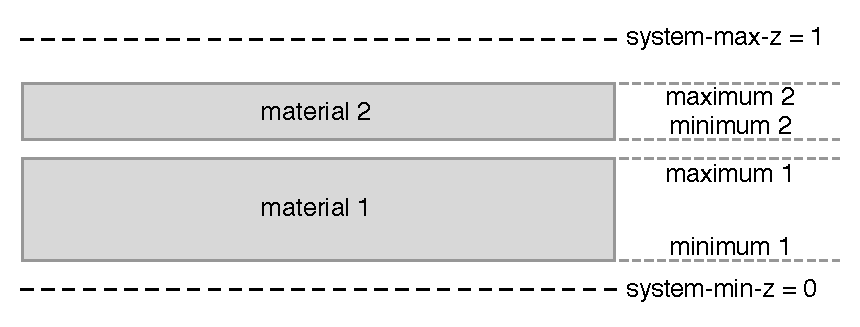
\includegraphics[width=7cm]{figures/multilayers.pdf}
\caption{Schematic diagram showing definition of a multilayer system consisting
of two materials. The minimum-height and maximum-height are defined as a
fraction of the total $z$-height of the system.}
\label{fig:multilayer}
\end{figure*}

The heights of the material are applied when the crystal is generated, and so
in general further geometry changes can also be applied, for example cutting a
cylinder shape or voronoi granular media, while preserving the multilayer
structure. The code will also print a warning if materials overlap their
minimum/maximum ranges, since such behaviour is usually (but not always)
undesirable.

{\zicf material:maximum-height = float [ 0-1 : default 1.0 ]}
\phantomsection\addcontentsline{toc}{subsection}{material:maximum-height}
Defines the maximum height of the material as a fraction of the total height
$z$ of the system. See material:minimum-height for more details.

{\zicf material:core-shell-size = float [ 0-1 : default 1.0 ]}
\phantomsection\addcontentsline{toc}{subsection}{material:core-shell-size}
Defines the radial extent of a material as a fraction of the particle radius.
This parameter is used to generate core-shell nanoparticles consisting of two
or more distinct layers.

\begin{figure*}[!htb]
\center
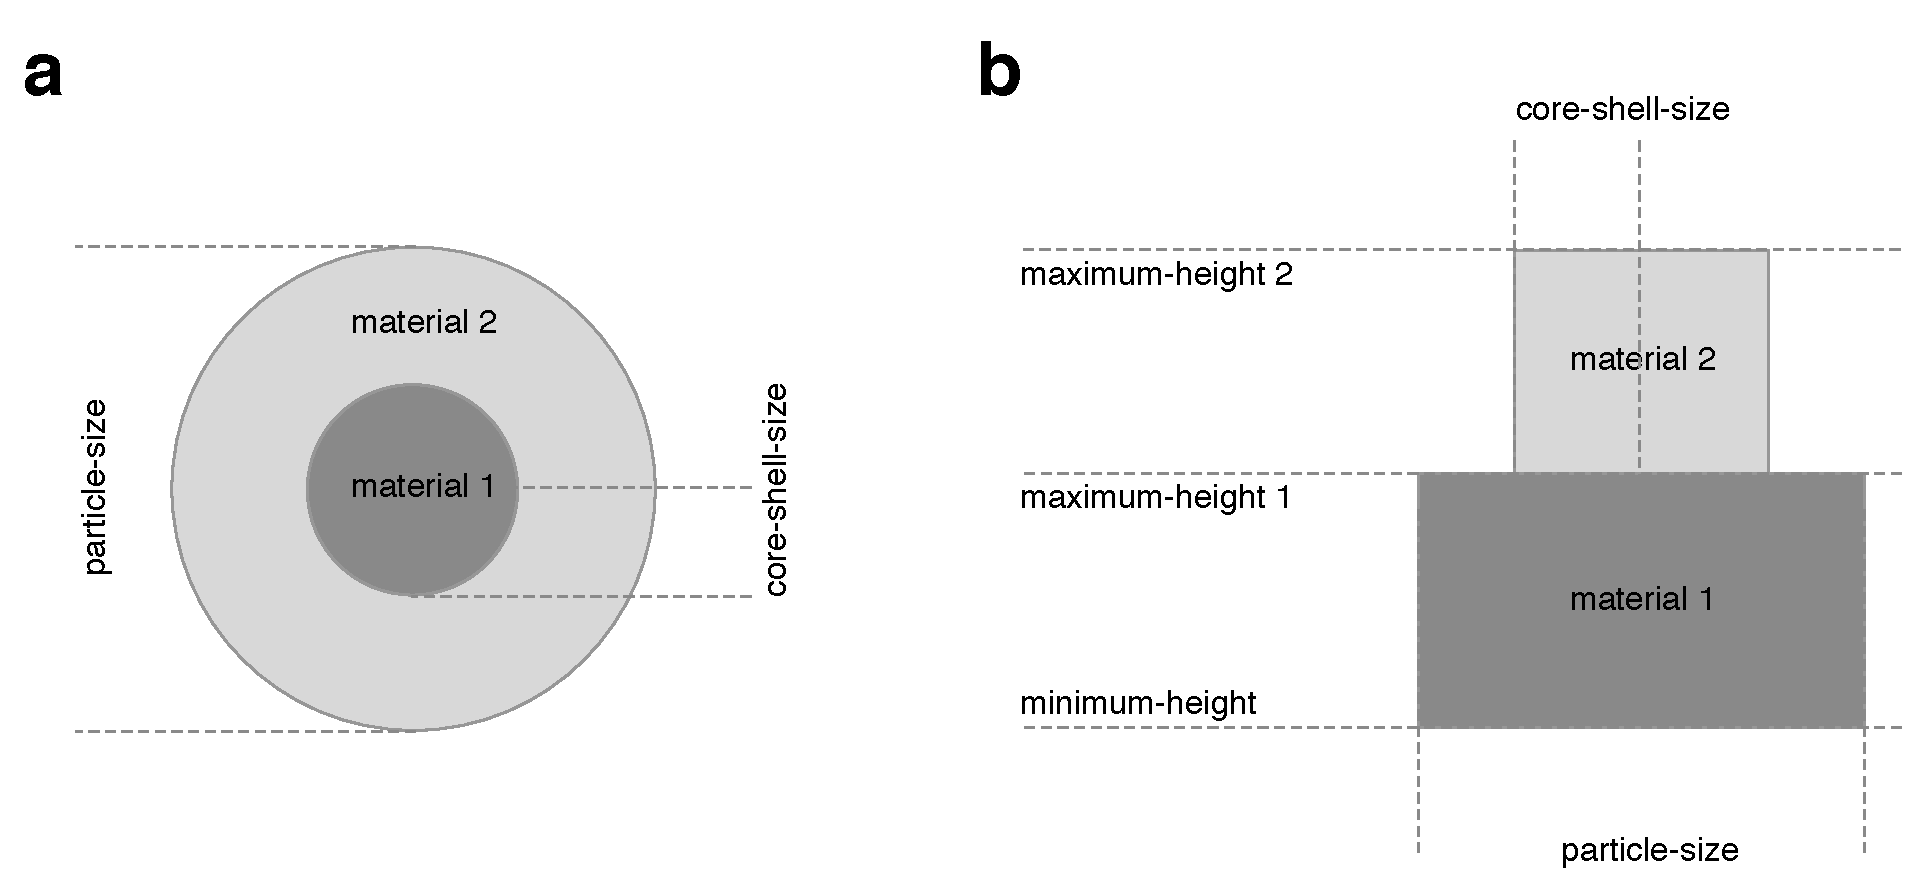
\includegraphics[width=10cm]{figures/core-shell.pdf}
\caption{\textbf{(a)} Schematic diagram showing definition of a nanoparticle
with two materials with different radii. core-shell-size is defined as a
fraction of the particle radius (particle-size/2). \textbf{(b)} Schematic
diagram showing side-on iew of a cylinder, consisting of two materials with
different core-shell-size and different maximum heights. Part of the core
material is exposed, while the other part is covered with the other material.}
\label{fig:core-shell}
\end{figure*}

The core-shell-size is compatible with spherical, ellipsoidal, cylindrical,
truncated octahedral and cuboid shaped particles. In addition when particle
arrays are generated all particles are also core-shell type. This option is
also comparable with the minimum/maximum-height options, allowing for partially
filled or coated nanoparticles.

{\zicf material:interface-roughness = float [ 0-1 : default 1.0 ]}
\phantomsection\addcontentsline{toc}{subsection}{material:interface-roughness}
Defines interfacial roughness in multilayer systems.

{\zicf material:intermixing[index] = float [ 0-1 : default 1.0 ]}
\phantomsection\addcontentsline{toc}{subsection}{material:intermixing}
Defines intermixing between adjacent materials in multilayer systems. The
intermixing is defined as a fraction of the total system height, and so small
values are usually used. The intermixing defines the mixing of material $index$
into the host material, and can be asymmetric (a -> b != b -> a).

{\zicf material:density = float [ 0-1 : default 1.0 ]}
\phantomsection\addcontentsline{toc}{subsection}{material:density} Defines the
fraction of atoms to remove randomly from the material (density).

{\zicf material:continuous = flag [ default off ]}
\phantomsection\addcontentsline{toc}{subsection}{material:continuous}
Defines materials which ignore granular CSG operations, such as particles,
voronoi media and particle arrays.

{\zicf material:fill-space = flag [ default off ]}
\phantomsection\addcontentsline{toc}{subsection}{material:fill-space}
Defines materials which obey granular CSG operations, such as particles,
voronoi media and particle arrays, but in-fill the void created. This is
useful for embedded nanoparticles and recording media with dilute interlayer
coupling.

{\zicf material:couple-to-phononic-temperature = flag [ default off ]}
\phantomsection\addcontentsline{toc}{subsection}{material:couple-to-phononic-temperature}
Couples the spin system of the material to the phonon temperature instead of the
electron temperature in pulsed heating simulations utilising the two temperature
model. Typically used for rare-earth elements.

{\zicf material:temperature-rescaling-exponent = float [ 0-10 : default 1.0 ]}
\phantomsection\addcontentsline{toc}{subsection}{material:temperature-rescaling-exponent}
Defines the exponent when rescaled temperature calculations are used. The higher
the exponent the flatter the magnetisation is at low temperature. This parameter
must be used with temperature-rescaling-curie-temperature to have any effect.

%-------------------------------------------------------------------------------
% STT
%-------------------------------------------------------------------------------
{\zicf material:spin-transfer-relaxation-torque = float [ default 0.0 T]}
\phantomsection\addcontentsline{toc}{subsection}{material:spin-transfer-relaxation-torque}
Defines the relaxational spin-transfer torque strength in terms of an effective
magnetic field in tesla. This is equivalent to the usual definition of the
(damping-like / anti-damping / Slonczewski) torque but without parasitic
components arising from the Landau-Lifshitz-Gilbert-Slonczewski (LLGS) equation
(see Andrea Meo \textit{et al}, J. Phys.: Condens. Matter 35 025801 (2023) for
more information about the implementation). The incoming spin-polarisation is
assumed to lie along the direction defined by
\textit{sim:spin-transfer-torque-spin-polarization-unit-vector} defined in the
\textit{input} file.

{\zicf material:spin-transfer-precession-torque = float [ default 0.0 T]}
\phantomsection\addcontentsline{toc}{subsection}{material:spin-transfer-precession-torque}
Defines the precessional spin-transfer torque strength in terms of an effective
magnetic field in tesla. This is equivalent to the usual definition of the
field-like torque but without parasitic components arising from the
Landau-Lifshitz-Gilbert-Slonczewski (LLGS) equation (see Andrea Meo
\textit{et al}, J. Phys.: Condens. Matter 35 025801 (2023) for more information
about the implementation). The incoming spin-polarisation is assumed to lie
along the direction defined by \textit{sim:spin-transfer-torque-spin-polarization-unit-vector}
defined in the \textit{input} file.

%-------------------------------------------------------------------------------
% SOT
%-------------------------------------------------------------------------------
{\zicf material:spin-orbit-relaxation-torque = float [ default 0.0 T]}
\phantomsection\addcontentsline{toc}{subsection}{material:spin-orbit-relaxation-torque}
Defines the relaxational spin-orbit torque strength in terms of an effective
magnetic field in tesla. This is equivalent to the usual definition of the
(damping-like) torque but without parasitic components arising from the
Landau-Lifshitz-Gilbert-Slonczewski (LLGS) equation (see Andrea Meo
\textit{et al}, J. Phys.: Condens. Matter 35 025801 (2023) for more information
about the implementation). The incoming spin-polarisation is assumed to lie
along the direction defined by \textit{sim:spin-orbit-torque-spin-polarization-unit-vector}
defined in the \textit{input} file.

{\zicf material:spin-orbit-precession-torque = float [ default 0.0 T]}
\phantomsection\addcontentsline{toc}{subsection}{material:spin-orbit-precession-torque}
Defines the precessional spin-orbit torque strength in terms of an effective
magnetic field in tesla. This is equivalent to the usual definition of the
field-like torque but without parasitic components arising from the
Landau-Lifshitz-Gilbert-Slonczewski (LLGS) equation (see Andrea Meo
\textit{et al}, J. Phys.: Condens. Matter 35 025801 (2023) for more information
about the implementation). The incoming spin-polarisation is assumed to lie
along the direction defined by \textit{sim:spin-orbit-torque-spin-polarization-unit-vector}
defined in the \textit{input} file.

{\zicf material:temperature-rescaling-curie-temperature = float [ 0-10,000 : default 0.0 ]}
\phantomsection\addcontentsline{toc}{subsection}{material:temperature-rescaling-curie-temperature}
Defines the Curie temperature of the material to which temperature rescaling is
applied.

{\zicf material:non-magnetic flag [default remove]}
\phantomsection\addcontentsline{toc}{subsection}{material:non-magnetic}
Defines atoms of that material as being non-magnetic. Non-magnetic atoms by
default are removed from the simulation and play no role in the simulation. If
configuration output is specified then the positions of the non-magnetic atoms
are saved and processed by the vdc utility. This preserves the existence of
non-magnetic atoms when generating visualisations but without needing to
simulate them artificially. The "keep" option preserves the non-magnetic atoms
in the simulation for parallelization efficiency but instructs the dipole field
solver to ignore them for improved accuracy.

%constrained // determines use of alternate integrator ?
%constraint-angle-theta
%constraint-angle-theta-min
%constraint-angle-theta-max
%constraint-angle-theta-delta
%constraint-angle-phi-min
%constraint-angle-phi
%constraint-angle-phi-max
%constraint-angle-phi-delta
%temperature
%fmr-field-strength
%fmr-field-frequency
%fmr-field-unit-vector
%applied-field-strength
%applied-field-unit-vector

{\zicf material:unit-cell-category = int [ default 0 ]}
\phantomsection\addcontentsline{toc}{subsection}{material:unit-cell-category}
Allocates different materials to different atoms in the unit cell. In complex
crystals such as spinel and rocksalt, the material allocations of
different atoms in the unit cell are defined by the structure. For example, in
the rocksalt structure there are two distinct types of atoms. Material 1 could
be allocated to this site using \textit{material[1]:unit-cell-category = 1},
and a second material could be allocated to the second site using
\textit{material[2]:unit-cell-category = 2}. The default value of this
variable is 0, and so for complex crystals only a single site is defined and
the other sites will not be generated unless a material is attached to it in
this way.

This keyword also works with the \textit{create:crystal-sublattice-materials}
flag to allocate different materials to different sites in the simple crystals
bcc, fcc, hcp and kagome. This feature is especially useful for simulating
simple antiferromagnets and materials with different kinds of defects or
site specific alloying.

%\section*{Example material files}
%\phantomsection\addcontentsline{toc}{section}{Example material files}

%\chapter{Chapter Title}\label{chap:modellingmethods}
%Some intro text\\

%\section*{Section Title}
%\phantomsection\addcontentsline{toc}{section}{Section Title}
%A section\\
%\subsection*{Subsection Title}
%A subsection\\







%
